\documentclass[10pt, landscape]{article}
\usepackage[scaled=0.92]{helvet}
\usepackage{calc}
\usepackage{multicol}
\usepackage[a4paper,margin=3mm,landscape]{geometry}
\usepackage{amsmath,amsfonts,amssymb}
\usepackage{color,graphicx,overpic}
\usepackage{hyperref}
\usepackage{newtxtext} 
\usepackage{enumitem}
\usepackage[table]{xcolor}
\usepackage{mathtools}
\usepackage{tikz}
\setlist{nosep}
% for including images
\graphicspath{ {../images/} }

\pdfinfo{
  /Title (ST2131.pdf)
  /Creator (TeX)
  /Producer (pdfTeX 1.40.0)
  /Author (Jovyn Tan)
  /Subject (ST2131)
/Keywords (ST2131, nus,cheatsheet,pdf)}

% Turn off header and footer
\pagestyle{empty}

% redefine section commands to use less space
\makeatletter
\renewcommand{\section}{\@startsection{section}{1}{0mm}%
  {-1ex plus -.5ex minus -.2ex}%
  {0.5ex plus .2ex}%x
{\normalfont\large\bfseries}}
\renewcommand{\subsection}{\@startsection{subsection}{2}{0mm}%
  {-1explus -.5ex minus -.2ex}%
  {0.5ex plus .2ex}%
{\normalfont\normalsize\bfseries}}
\renewcommand{\subsubsection}{\@startsection{subsubsection}{3}{0mm}%
  {-1ex plus -.5ex minus -.2ex}%
  {1ex plus .2ex}%
{\normalfont\small\bfseries}}%
\makeatother

\renewcommand{\familydefault}{\sfdefault}
\renewcommand\rmdefault{\sfdefault}
%  makes nested numbering (e.g. 1.1.1, 1.1.2, etc)
\renewcommand{\labelenumii}{\theenumii}
\renewcommand{\theenumii}{\theenumi.\arabic{enumii}.}
\renewcommand\labelitemii{•}
\renewcommand\labelitemiii{•}

\definecolor{mathblue}{cmyk}{1,.72,0,.38}
\everymath\expandafter{\the\everymath \color{mathblue}}

% Don't print section numbers
\setcounter{secnumdepth}{0}

%% adjust spacing for all itemize/enumerate
\setlength{\leftmargini}{0.5cm}
\setlength{\leftmarginii}{0.5cm}
\setlist[itemize,1]{leftmargin=2mm,labelindent=1mm,labelsep=1mm}
\setlist[itemize,2]{leftmargin=4mm,labelindent=1mm,labelsep=1mm}

% adding my commands
% tightcenter
\newenvironment{tightcenter}{%
  \setlength\topsep{0pt}
  \setlength\parskip{0pt}
  \begin{center}
    }{%
  \end{center}
}

% boxed
\newenvironment{tightbox}{%
  \setlength\topsep{0pt}
  \setlength\parskip{0pt}
  \begin{center}
    \begin{tabular}{|@{\hspace{\dimexpr\fboxsep+0.5\arrayrulewidth}}c@{\hspace{\dimexpr\fboxsep+0.5\arrayrulewidth}}|}
      \hline
    }
    {%
    \\ \hline
    \end{tabular}
  \end{center}
}

% fixed width box
\newenvironment{fixedbox}[1][0.7]{
  \setlength\topsep{0pt}
  \setlength\parskip{0pt}
  \begin{center}
    \begin{tabular}{|>{\centering\arraybackslash}m{#1\linewidth}|}
    \hline
  }{
  \\ \hline
  \end{tabular}
  \end{center}
}

% definition of a new term
\usepackage{soul}
\definecolor{paleyellow}{RGB}{251,243,218}
\newcommand{\definition}[2][]{\sethlcolor{paleyellow}\hl{\textbf{#2}} #1  $\rightarrow$}
% inline definition
\newcommand{\ildefinition}[1]{\sethlcolor{paleyellow}\hl{\textbf{#1}}}

% important note (attention)
\newcommand{\attention}{{\color{red}\textbf{! }}}

% nice proof
\newenvironment{niceproof}[1][Proof]
{%
  \sbox0{\textit{#1}. }%
  \list{}{\labelwidth\wd0 \leftmargin\wd0 \labelsep 0pt }
\item[\usebox0]}
  {\endlist}


%  convenient absolute value symbol
\newcommand{\abs}[1]{\vert #1 \vert}

%  convenient floor and ceiling
\newcommand{\floor}[1]{\lfloor #1 \rfloor}
\newcommand{\ceil}[1]{\lceil #1 \rceil}

%  modulo with nicer spacing
\newcommand{\Mod}[1]{\ \mathrm{mod}\ #1}

%  convenient dx with nicer spacing
\newcommand{\dx}{\mathop{dx}}
\newcommand{\dy}{\mathop{dy}}



% -----------------------------------------------------------------------

\begin{document}
\raggedright
\footnotesize

% space above/below equation environment 
\setlength{\abovedisplayskip}{1pt}
\setlength{\belowdisplayskip}{1pt}

\begin{multicols*}{3}
  % multicol parameters
  \setlength{\columnseprule}{0.25pt}

  \begin{center}
    \fbox{%
      \parbox{0.8\linewidth}{\centering \textcolor{black}{
          {\Large\textbf{ST2131}}
        \\ \normalsize{AY21/22 SEM 2}}
        \\ {\footnotesize \textcolor{gray}{github/jovyntls}}
      }%
    }
  \end{center}

  \section{01. COMBINATORIAL ANALYSIS}

  \subsection{The Basic Principle of Counting}

  \begin{itemize}
    \item \definition{basic principle of counting} Suppose that two experiments are performed. 
      If exp1 can result in any one of $m$ possible outcomes and if, for each outcome of exp1, there are $n$ possible outcomes of exp2, 
      then together there are $mn$ possible outcomes of the two experiments.
    \item \definition{generalized basic principle of counting} If $r$ experiments are performed such that the first one may result in any of $n_1$ possible outcomes and if for each of these $n_1$ possible outcomes, there are $n_2$ possible outcomes of the 2nd exp, and if ..., then there is a total of $n_1 \cdot n_2 \cdot \dots \cdot n_r$ possible outcomes of $r$ experiments.
  \end{itemize}

  \subsection{Permutations}

  \textbf{factorials} - $1! = 0! = 1$

  \textbf{N1} - if we know how to count the number of different ways that an event can occur, we will know the probability of the event.

  \textbf{N2} - there are $n!$ different arrangements for $n$ objects.

  \textbf{N3} - there are $\frac{n!}{n_1!\, n_2!\, \dots n_r!}$ different arrangements of $n$ objects, 
  of which $n_1$ are alike, $n_2$ are alike, ..., $n_r$ are alike.

  \subsection{Combinations}

  \begin{tightcenter}
    $\binom{n}{r} = \frac{n!}{(n-r)!\,r!} = \binom{n-1}{r-1} + \binom{n-1}{r}, \quad 1 \leq r \leq n$
  \end{tightcenter}

  \textbf{N5} - \textbf{The Binomial Theorem}
  \begin{tightcenter}
    \( {\displaystyle{(x+y)^n = \sum^n_{k=0} \binom{n}{k} x^k y^{n-k} }} \) 
  \end{tightcenter}

  \subsection{Multinomial Coefficients}

  \begin{tightcenter}
    $\binom{n}{n_1, n_2, \dots, n_r} = \frac{n!}{n_1!\, n_2!\, \dots \, n_r!}$  
  \end{tightcenter}

  \textbf{N6} - represents the number of possible divisions of $n$ distinct objects 
  into $r$ distinct groups of respective sizes $n_1, n_2, \dots, n_3$, 
  where $n_1 + n_2 + \dots + n_r = n$

  \textbf{N7} - \textbf{The Multinomial Theorem}: $(x_1 + x_2 + \dots + x_r)^n$
  \\* $ \quad\quad\quad = \sum\limits_{(n_1, \dots, n_r):n_1 + n_2 + \dots + n_r = n} \frac{n!}{n_1! \, n_2! \, \dots n_r!} x_1^{n_1} x_2^{n_2} \dots x_r^{n_r}$

  \subsection{Number of Integer Solutions of Equations}

  \textbf{N8} - there are $\binom{n-1}{r-1}$ distinct \textit{positive} integer-valued vectors $(x_1, x_2, \dots, x_r)$ satisfying
  $x_1 + x_2 + \dots + x_r = n, \quad x_i > 0, \quad i = 1,2,\dots,r$  

  \textbf{N9} - there are $\binom{n+r-1}{r-1}$ distinct  \textit{non-negative} integer-valued vectors $(x_1, x_2, \dots, x_r)$ satisfying $x_1 + x_2 + \dots + x_r = n$ 
  \begin{niceproof}
    let $y_k = x_k + 1 \Rightarrow y_1 + y_2 + \dots + y_r = n + r$
  \end{niceproof}


  \section{02. AXIOMS OF PROBABILITY}

  \subsection{Sample Space and Events}
  \begin{itemize}
    \item \definition{sample space} The \textit{set} of all outcomes of an experiment 
    \item \definition{event} Any \textit{subset} of the sample space
    \item \definition[of $E$]{complement} $E^c$ is the event that contains all outcomes that are \textit{not} in $E$.
    \item \definition{subset} $E \subset F$ is all of the outcomes in $E$ that are also in $F$.
      \begin{itemize}
        \item $E \subset F \land F \subset E \Rightarrow E = F$
      \end{itemize}
  \end{itemize}

  \textbf{DeMorgan's Laws}:
  $\quad\quad \mathbf{ (\bigcup\limits^n_{i=1} E_i)^c = \bigcap\limits^n_{i=1}E_i^c } \quad$ and $\quad \mathbf{ (\bigcap\limits^n_{i=1}E_i)^c = \bigcup\limits^n_{i=1}E_i^c }$ \\

  \subsection{Axioms of Probability}

  \textbf{definition 1: relative frequency}

  $P(E) = \lim_{n \to \infty} \frac{n(E)}{n}$. $\quad$ problems: (1) $\frac{n(E)}{n}$ may not converge when $n \to \infty$. (2) $\frac{n(E)}{n}$ may not converge to the same value if the experiment is repeated.

  \subsubsection{Axioms (definition 2)}

  Consider an experiment with sample space $S$. 
  For each event $E$ of the sample space $S$, we assume that a number $P(E)$ is defined and satisfies the following 3 axioms:

  1. $0 \leq P(E) \leq 1$ 
  $\quad\quad\quad\quad$
  2. $P(S) = 1$

  3. For mutually exclusive events, $P(\bigcup\limits^\infty_{i=1} E_i) = \sum\limits^\infty_{i=1} P(E_i)$. $\quad$ same for finite case

  \definition{mutually exclusive} events for which $E_iE_j = \emptyset$ when  $i \neq j$

  \subsection{Simple Propositions}

  \textbf{N1} - $P(\emptyset) = 0$

  \textbf{N6} - \textbf{probability function} $\iff$ it satisfies the 3 axioms.

  \textbf{N8} - if $E \subset F$, then $P(E) \leq P(F)$

  \textbf{N10} - Inclusion-Exclusion identity where $n=3$
  $P(E \cup F \cup G) = P(E) + P(F) + P(G) - P(EF) - P(EG) - P(FG) + P(EFG)$

  \textbf{N11} - \textbf{Inclusion-Exclusion identity} - 

  ${\scriptstyle P(E_1 \cup E_2 \cup \dots \cup E_n) = \sum\limits^n_{i=1} P(E_i) - \sum\limits_{i_1 < i_2} P(E_{i_1} E_{i_2}) + \dots }$ 
  ${\scriptstyle + (-1)^{r+1} \sum\limits_{i_1 < i_2 < \dots < i_r} P(E_{i_1} E_{i_2} \dots E_{i_r}) + \; \dots \; + (-1)^{n+1} P(E_1 E_2 \dots E_n) }$

  \begin{enumerate}[label=(\roman*)]
    \item $P(\bigcup^n_{i=1}E_i) \leq \sum\limits^n_{i=1} P(E_i)$ (based on Inclusion-Exclusion identity)
    \item $P(\bigcup^n_{i=1}E_i) \geq \sum\limits^n_{i=1} P(E_i) - \sum\limits_{j < i} P(E_iE_j)$
    \item $P(\bigcup^n_{i=1}E_i) \leq \sum\limits^n_{i=1} P(E_i) - \sum\limits_{j < i} P(E_iE_j) + \sum_{k < j < i} P(E_iE_jE_k)$
    \item and so on.
  \end{enumerate}


  \subsection{Sample Space having Equally Likely Outcomes}

  Consider an experiment with sample space $S = \{e_1, e_2, \dots, e_n\}$. 
  Then  $P(\{e_1\}) = P(\{e_2\}) = \dots = P(\{e_n\}) = \frac{1}{n} \quad$ or $\quad P(\{e_i\}) = \frac{1}{n}$.

  \textbf{N1} - for any event $E$, $P(E) = \frac{\# \text{ of outcomes in } E}{\# \text{ of outcomes in } S}  = \frac{\# \text{ of outcomes in } E}{n} $

  \ildefinition{increasing sequence} of events $\{E_n, n \geq 1\}$ $\rightarrow$ $E_1 \subset E_2 \subset \dots \subset E_n \subset \dots$


  \ildefinition{decreasing sequence} of events $\{E_n, n \geq 1\}$ $\rightarrow$ $E_1 \supset E_2 \supset \dots \supset E_n \supset \dots$

  increasing: $\lim\limits_{n \to \infty} E_n = \bigcup\limits^\infty_{i=1}E_i$ $\quad\quad$
  decreasing: $\lim\limits_{n \to \infty} E_n = \bigcap\limits^\infty_{i=1}E_i$

  \textbf{N2} - for both \textit{increasing} and \textit{decreasing} sequence, 
  $\lim\limits_{n \to \infty} P(E_n) = P(\lim\limits_{n \to \infty} E_n)$


  \section{03. CONDITIONAL PROBABILITY AND INDEPENDENCE}

  \subsection{Conditional Probability}

  \begin{tightcenter}
    if $P(F) > 0$, then $P(E|F) = \frac{P(E \cap F)}{P(F)} $

    \textbf{multiplication rule}:

    $P(E_1\dots E_n) = P(E_1)P(E_2\vert E_1)P(E_3\vert E_1 E_2) \dots P(E_n \vert E_1 E_2 \dots E_{n-1})$
  \end{tightcenter}

  \textbf{N3} - \textbf{axioms of probability} apply to conditional probability

  1.  $ 0 \leq P(E \vert F) \leq 1 $ $\quad\quad\quad\quad$
  2. $ P(S \vert F) = 1 $ where $ S $ is the sample space

  3. If $ E_i $ ($ i \in \mathbb{Z}_{\geq 1} $) are mutually exclusive, then $ P(\bigcup\limits^\infty_1 E_i \vert F) = \sum\limits^\infty_1 P(E_i \vert F) $

  \textbf{N4} - If we define $ Q(E) = P(E \vert F) $, 
  then all previously proven results apply.
  \begin{itemize}
    \item $P(E_1\cup E_2\vert F ) = P(E_1\vert F ) + P(E_2\vert F ) - P(E_1 E_2\vert F ) $ 
  \end{itemize}


  \subsection{Total Probability \& Bayes' Theorem}

  \textbf{conditioning formula} - $P(E) = P(E \vert F)P(F) + P(E\vert F^c) P(F^c)$

  \begin{minipage}[c]{0.4\linewidth}
    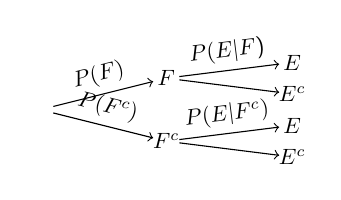
\begin{tikzpicture}[scale=0.8, every node/.style={transform shape}]
      \node[minimum size=4mm, inner sep=0] (O) at (0,1.25) {};
      \node[label=center:{$F$}, minimum size=4mm, inner sep=0] (F) at (2,1.75) {};
      \node[label=center:{$F^c$}, minimum size=4mm, inner sep=0] (Fc) at (2,0.75) {};
      \node[label=center:{$E$}, minimum size=4mm, inner sep=0] (FE) at (4,2) {};
      \node[label=center:{$E^c$}, minimum size=4mm, inner sep=0] (FEc) at (4,1.5) {};
      \node[label=center:{$E$}, minimum size=4mm, inner sep=0] (FcE) at (4,1) {};
      \node[label=center:{$E^c$}, minimum size=4mm, inner sep=0] (FcEc) at (4,0.5) {};
      \draw[->] (F) -- (FE) node[midway, above, sloped] {$P(E\vert F$)};
      \draw[->] (F) -- (FEc) node[midway, above, sloped] {};
      \draw[->] (Fc) -- (FcE) node[midway, above, sloped] {$P(E\vert F^c)$};
      \draw[->] (Fc) -- (FcEc) node[midway, above, sloped] {};
      \draw[->] (O) -- (F) node[midway, above, sloped] {$P(F)$};
      \draw[->] (O) -- (Fc) node[midway, above, sloped] {$P(F^c)$};
    \end{tikzpicture}
  \end{minipage}
  \begin{minipage}[c]{0.55\linewidth}
    $P(F \vert E) = \frac{P(EF)}{P(E)} = \frac{P(F) \cdot P(E \vert F)}{P(E)}$ \\
    $P(F^c \vert E) = \frac{P(EF^c)}{P(E)} = \frac{P(F^c) \cdot P(E \vert F^c)}{P(E)}$ 
  \end{minipage}

  \subsubsection{Total Probability}

  \textbf{theorem of total probability} - 
  Suppose $F_1, F_2, \dots, F_n$ are mutually exclusive events such that $\bigcup\limits^n_{i=1}F_i = S$, 
  then $P(E) = \sum\limits^n_{i=1}P(EF_i) = \sum\limits^n_{i=1}P(F_i)P(E\vert F_i)$

  \subsubsection{Bayes Theorem}
  \begin{tightcenter}
    $P(F_j \vert E) = \frac{P(EF_j)}{P(E)} = \frac{P(F_j)P(E \vert F_j)}{\sum\limits^n_{i=1} P(F_i)P(E \vert F_i)}$
  \end{tightcenter}

  \textbf{application of bayes' theorem}

  \begin{tightcenter}
    $P(B_1 \mid A) = \frac{P(A \mid B_1) \cdot P(B_1)}{P(A \mid B_1) \cdot P(B_1) + P(A \mid B_2) \cdot P(B_2)}$
  \end{tightcenter}

  Let $A$ be the event that the person test positive for a disease.
  \\* $B_1$: the person has the disease. $B_2$: the person does not have the disease.
  \begin{tightcenter}
    \vspace*{-1\multicolsep}
    \begin{multicols}{2}
      true positives: $P(B_1\mid A)$
      \\ false positives: $P(A \mid B_2)$
      \\ false negatives: $P(\bar{A} \mid B_1)$
      \\ true negatives: $P(\bar{A} \mid B_2)$
    \end{multicols}
    \vspace*{-1\multicolsep}
  \end{tightcenter}

  \subsection{Independent Events}

  \textbf{N1} - $E$ and $F$ are independent $\iff P(EF) = P(E) \cdot P(F) \quad$ 

  \textbf{N2} - $E$ and $F$ are independent $\iff P(E \vert F) = P(E)$

  \textbf{N3} - $E$ and $F$ are independent $\iff$ $E$ and $F^c$ are independent.

  \textbf{N4} - if $E, F, G$ are independent, then $E$ will be independent of any event formed from $F$ and $G$. (e.g. $F\cup G$)

  \textbf{N6} - ($ E $ and $ F $ are indep) $\land$ ($ E $ and $ G $ are indep) 
  $\not\Rightarrow $  $ E $ and $ FG $ are independent

  \textbf{N7} - For independent trials with probability $ p $ of success, probability of $ m $ successes before $ n $ failures, 
  for $ m, n \geq 1 $,

  \begin{minipage}[c]{0.3\linewidth}
    \textit{method 1}\\
    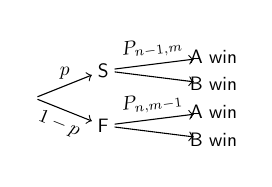
\begin{tikzpicture}[scale=0.7, every node/.style={transform shape}]
      \node[minimum size=1mm, inner sep=0] (O) at (0,1.25) {};
      \node[label=center:{S}, minimum size=4mm, inner sep=0] (S) at (1.25,1.75) {};
      \node[label=center:{F}, minimum size=4mm, inner sep=0] (F) at (1.25,0.75) {};
      \node[label=center:{A win}, minimum size=7mm, inner sep=0] (a1) at (3.25,2) {};
      \node[label=center:{B win}, minimum size=7mm, inner sep=0] (b1) at (3.25,1.5) {};
      \node[label=center:{A win}, minimum size=7mm, inner sep=0] (a2) at (3.25,1) {};
      \node[label=center:{B win}, minimum size=7mm, inner sep=0] (b2) at (3.25,0.5) {};
      \draw[->] (S) -- (a1) node[midway, above, sloped] {$P_{n-1, m}$};
      \draw[->] (S) -- (b1) node {};
      \draw[->] (F) -- (a2) node[midway, above, sloped] {$P_{n, m-1}$};
      \draw[->] (F) -- (b2) node {};
      \draw[->] (O) -- (S) node[midway, above] {$p$};
      \draw[->] (O) -- (F) node[midway, below, sloped] {$1-p$};
    \end{tikzpicture}
  \end{minipage}
  \begin{minipage}[c]{0.67\linewidth}
    \textit{method 2}
    \begin{align*}
      P_{n, m} &= \sum\limits^{m+n-1}_{k=n} \binom{m+n-1}{k} p^k (1-p)^{m+n-1-k} 
            \\ &= P(\text{$\geq n$ successes in $ m+n-1 $ trials})
    \end{align*}
  \end{minipage}


  \section{04. RANDOM VARIABLES}

  \begin{itemize}
    \item \definition{random variable} a real-valued function defined on the sample space
  \end{itemize}

  \subsection{Types of Random Variables}

  \begin{tabular}{|c|l|c|}
    \hline  \textbf{r.v.} & - & $E(X)$
    \\\hline  binomial & $ X= $ \# of successes in $ n $ trials w/ replacement & $ np$
    \\\hline negative binomial & $ X= $ \# of trials until $ k $ successes & $k/p$
    \\\hline geometric & $ X= $ \# of trials until a success & $1/p$
    \\\hline hypergeometric & $ X= $ \# of successes in $ n $ trials, no replacement & $rn/N$
    \\\hline
  \end{tabular}

  \begin{itemize}
    \item $X$ is a \definition[with parameter $p$ if]{Bernoulli r.v.} 
      \\* $\quad p(x) = \begin{cases}
        p, &x=1, \text{ ('success')} \\
        1-p, &x=0\quad  \text{ ('failure')}
      \end{cases}$
    \item $ Y $ is a \definition[with parameters $ n $ and $ p $]{Binomial r.v.} $ \quad Y = X_1 + X_2 + \dots + X_n $
      where  $ X_1, X_2, \dots, X_n $ are independent Bernoulli r.v.'s with parameter $ p $.
      \begin{itemize}
        \item $ P(X=k) = \binom{n}{k} p^k (1-p)^{n-k} $
        \item $ P(k $ successes from $ n $ independent trials each with probability $ p $ of success$ ) $
      \end{itemize}
      \centerline{$E(Y) = np, \quad Var(Y) = np(1-p)$}
    \item \definition{Negative Binomial} $ X = $ number of trials until $ k $ successes are obtained
      \begin{itemize}
        \item e.g. number of balls drawn (with replacement) until $ k $ red balls are obtained
      \end{itemize}
    \item \definition{Geometric} $ X = $ number of trials until a success is obtained
      \begin{itemize}
        \item $ P(X=k) = (1-p)^{k-1} \cdot p $ where $ k $ is the number of trials needed
        \item e.g. number of balls drawn (with replacement) until 1 red ball is obtained
      \end{itemize}
    \item \definition{Hypergeometric} $ X = $ number of trials until success, \textit{without replacement}
      \begin{itemize}
        \item $P(X=k) = \frac{\binom{m}{k}\binom{N-m}{n-k}}{\binom{N}{n}}$, $k = 0,1,\dots, n \quad$ (for $m$ red balls of $N$ balls)
        \item e.g. number of red balls out of $ n $ balls drawn without replacement
      \end{itemize}
  \end{itemize}

  \subsubsection{Properties}

  \textbf{N1} - if $X \sim \text{Binomial}(n,p)$, and $Y \sim \text{Binomial}(n-1, p)$, then
  \\* \centerline{$E(X^k) = np \cdot E[(Y+1)^{k-1}]$}

  \textbf{N2} - if $X \sim \text{Binomial}(n,p)$, then for $k \in \mathbb{Z}^+$, 
  \\* \centerline{$P(X=k) = \frac{(n-k+1)p}{k(1-p)} \cdot P(X=k-1)$}

  \subsubsection{Coupon Collector Problem}

  \begin{niceproof}[Q]
    Suppose there are $ N $ distinct types of coupons.
    If $ T $ denotes the number of coupons needed to be collected for a complete set, what is $ P(T=n) $?
  \end{niceproof}

  \begin{niceproof}[A]
    $ P(T > n-1) = P(T \geq n) = P(T=n) + P(T > n) $
    $ \quad\Rightarrow P(T=n) = P(T > n-1) - P(T > n) $

    Let $ A_j = \{ \text{no type $j$ coupon is contained among the first $n$} \} $
    $ P(T>n) = P(\bigcup^N_{j=1}A_j) $

    $  P(T>n) = \sum_j P(A_j)\quad$ - coupon $ j $ is not among the first $ n $ collected 
    \\* $\quad\quad\quad\quad\quad - \sum\sum_{j_1<j_2} P(A_{j_1} A_{j_2}) \quad$ - coupon $ j_1 $ and $ j_2 $ are not the first $ n $
    \\* $\quad\quad\quad\quad\quad + \dots +  (-1)^{N+1} P(A_1A_2 \cdots A_N) $ by \textit{inclusion-exclusion identity}

    $ P(A_{j_1}A_{j_2} \cdots A_{j_k}) = ( \frac{N-k}{N} )^n $

    Hence $ P(T>n) = \sum\limits^{N-1}_{i=1} \binom{N}{i} (\frac{N-i}{N})^n (-1)^{i+1} $
  \end{niceproof}

  \subsection{Probability Mass Function}

  \definition[, pmf of $X$ (\textit{discrete})]{probability mass function} $\quad p(a) = P(X=a) $
  \begin{itemize}
    \item if $X$ assumes one of the values $x_1, x_2, \dots$, then $\sum^\infty_{i=1} p(x_i) = 1$
  \end{itemize}

  \subsection{Cumulative Distribution Function}
  \begin{itemize}
    \item \definition[of a r.v. $X$]{cumulative distribution function (cdf)} the function $F$ defined by $\quad\quad F(x) = P(X \leq x), \quad -\infty < x < \infty$
      \begin{itemize}
        \item $F(x)$ is defined on the entire real line. (aka \textit{distribution function})
      \end{itemize}
  \end{itemize}

  \begin{minipage}[c]{0.45\linewidth}
    \begin{tightcenter}
      \textbf{pmf},
      $\begin{array}{c|ccc}
        a & 1 & 2 & 4 \\\hline
        p(a) & \frac{1}{2} & \frac{1}{4} & \frac{1}{4} 
      \end{array}$

      \ \\
      $F(a) = \sum p(x)$ for all $x \leq a$
    \end{tightcenter}
  \end{minipage}
  \begin{minipage}[c]{0.45\linewidth}
    \begin{tightcenter}
      \textbf{cdf},
      $F(a) = \begin{cases}
        0, &a < 1 \\
        1/2, &1 \leq a < 2 \\
        3/4, &2 \leq a < 4 \\
        1, &a \geq 4
      \end{cases}$
    \end{tightcenter}
  \end{minipage}

  \subsection{Expected Value}
  \begin{itemize}
    \item aka population mean/sample mean, $\mu$
  \end{itemize}

  \begin{tightcenter}
    \textit{discrete}: $E(X) = \sum_x x \cdot p(x)$

    \textit{continuous}: $E(X) = \int^\infty_{-\infty} x \cdot f(x) \dx$

    $E[g(x)] = \int\limits^\infty_{-\infty} g(x) f(x) \dx $
  \end{tightcenter}

  \textbf{N1} - if $a$ and $b$ are constants, then $E(aX + b) = aE(X) + b$

  \textbf{N3} - for a non-negative r.v. $Y$, $E(Y) = \int^\infty_0 P(Y > y) \mathop{dy}$

  \begin{niceproof}
    $\int^\infty_0 P(Y > y) \dy = \int^\infty_0 \int^\infty_y f_Y(x) \dx \dy$ (because $f(x) = \frac{d}{\dx} F(x) $)
    \\* = $\int^\infty_0 x f_Y(x) \dx \quad = E(Y)$
  \end{niceproof}

  \begin{itemize}
    \item $I$ is an indicator variable for event $A$ if 
      $I = \begin{cases}\scriptstyle 1, \text{ if $A$ occurs} \\ \scriptstyle 0, \text{ if $A^c$ occurs}\end{cases}$. then $E(I) = P(A)$.
  \end{itemize}

  \subsubsection{finding expectation of f(x)}

  \begin{itemize}
    \item method 1, using pmf of $Y$: let $Y = f(X)$. Find corresponding $X$ for each $Y$.
    \item method 2, using pmf of $X$: $E[f(x)] = \sum_x f(x)p(x)$
  \end{itemize}

  \subsection{Variance}

  If $X$ is a r.v. with mean $\mu = E[X]$, then the \ildefinition{variance} of $X$ is defined by 
  \begin{align*}
    Var(X) &= E[(X-\mu)^2] \\[-0.5em] 
           &= E(x^2) - [E(x)]^2
  \end{align*}

  \begin{itemize}
    \item $Var(aX+b) = a^2 Var(x)$
      \item $Var(X) = \sum_{x_i} (x_i - \mu)^2 \cdot p(x_i) \quad\quad \text{(deviation $\cdot$ weight)}$
  \end{itemize}

  \subsection{Poisson Random Variable}

  a r.v. $X$ is said to be a \ildefinition{Poisson r.v.} with parameter $\lambda$ if for some $\lambda > 0$, 
  \begin{tightcenter}
    $ P(X=i) = e^{-\lambda} \cdot \frac{\lambda^i}{i!} $

    $E(X) = \lambda, \quad Var(X) = \lambda$
  \end{tightcenter}

  \begin{itemize}
    \item $\sum^\infty_{i=0} P(X=i) = 1$
    \item \textbf{Poisson Approximation of Binomial} - if $X \sim \text{Binomial}(n,p)$, where $n$ is large and $p$ is small, then $X \dot\sim \text{Poisson}(\lambda)$ where $\lambda=np$.
      \begin{itemize}
        \item $\checkmark$  \textit{weak} dependence is ok 
      \end{itemize}
    \item \textbf{2 ways} to look at the Poisson distribution 
      \begin{enumerate}
        \item an approximation to the binomial distribution with large $n$ and small $p$
        \item counting the number of events that occur at \textit{random} at certain points in time
      \end{enumerate}
  \end{itemize}

  \subsection{Poisson distribution as random events}

  Let $N(t)$ be the number of events that occur in time interval $[0, t]$. 

  \textbf{N1} - If the 3 assumptions are true, then  $N(t) \sim \text{Poisson}(\lambda t)$.

  \textbf{N2} - If $\lambda$ is the \textit{rate of occurrences} of events per unit time, then the number of occurrences in an interval of length $t$ has a Poisson distribution with mean $\lambda t$.

  \begin{tightcenter}
    $P(N(t) = k) = \frac{e^{-\lambda t} (\lambda t)^k}{k!} $, for $k \in \mathbb{Z}_{\geq 0}$
  \end{tightcenter}

  \subsubsection{o(h) notation}

  \begin{tightcenter}
    $o(h)$ stands for any function $f(h)$ such that \( {\displaystyle{ \lim_{h \to 0} \frac{f(h)}{h} = 0 }} \) 
  \end{tightcenter}

  \begin{itemize}
    \item $o(h) + o(h) = o(h)$
    \item $ \frac{\lambda t}{n} + o ( \frac{t}{n} ) \dot= \frac{\lambda t}{n} $ for large $n$
  \end{itemize}

  \subsection{Expected Value of sum of r.v.}

  For a r.v. $X$, let $X(s)$ denote the value of $X$ when $s \in \mathcal{S}$

  \textbf{N1} - $E(x) = \sum\limits_i x_i P(X=x_i) = \sum\limits_{s \in \mathcal{S}} X(s) p(s)$
  where $\mathcal{S}_i = \{s : X(s)=x_i\}$

  \textbf{N2} - $E (\sum\limits_{i-1}^n) = \sum\limits^n_{i=1}E(X_i) \quad$ for r.v. $X_1, X_2, \dots, X_n$

  \subsubsection{e.g. distribution of time to next event}

  Q. suppose an accident happens at a rate of 5 per day. Find the distribution of time, starting from now, until the next accident.

  \begin{niceproof}[A]
    Let $X =$ time (in days) until the next accident.
    \\* Let $V =$ be the number of accidents during time period $[0, t]$. 
    \\* $V \sim \text{Poisson}(5t) \quad \quad \Rightarrow P(V=k) = \frac{e^{-5t} \cdot (5t)^k}{k!} $

    $P(X > t) = P($no accidents happen during $[0, t]) = P(V=0) = e^{-5t}$

    $P(X \leq t) - 1-e^{-5t}$
  \end{niceproof}

  \subsubsection{example: finding pdf}

  \textit{Q} - Find the pdf of $(b-a)X + a$ where $a, b$ are constants, $b>a$.
  The pdf of $X$ is given by $f(x) =  \begin{cases} 1, &0 \leq X \leq 1 \\ 0, &\text{otherwise} \end{cases}$. 

  \begin{niceproof}[A]
    Let $Y = (b-a)X + a$. 
    \\* cdf, $F_Y(y) = P(Y \leq y) = P((b-a)X + a \leq y) = P(X \leq \frac{y-a}{b-a})$
    \\* $F_Y(y) = \int^{\frac{y-a}{b-a}}_0 1 \dx = \frac{y-a}{b-a}, \quad a < y < b $

    $f_Y(y) = \frac{d}{dy}F_Y(y) = \begin{cases} \frac{1}{b-a}, &a<y<b \\ 0, &\text{otherwise} \end{cases}$
  \end{niceproof}


  \section{05. CONTINUOUS RANDOM VARIABLES}

  $X$ is a \definition{continuous r.v.} if there exists a nonnegative function $f$ defined for all real $x \in (-\infty, \infty)$, 
  such that $P(X \in B) = \int_B f(x) \dx$ 

  \begin{minipage}[c]{0.6\linewidth}
    \textbf{N1} - $P(X \in (-\infty, \infty)) = \int^\infty_{-\infty} f(x) \dx = 1 $

    \textbf{N2} - $P(a \leq X \leq b) = \int^b_a f(x) \dx$

    \textbf{N3} - $P(X=a) = \int^a_a f(x) \dx = 0$

    \textbf{N4} - $P(X < a) = P(X \leq a) = \int^a_{-\infty} f(x) \dx$
  \end{minipage}
  \begin{minipage}[c]{0.35\linewidth}
    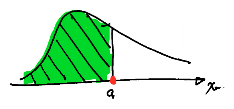
\includegraphics[width=0.9\linewidth]{st2131-continuous-rv-fx.png} 
  \end{minipage}

  \textbf{N5} - interpretation of \textbf{probability density function} 

  \begin{minipage}[c]{0.4\linewidth}
    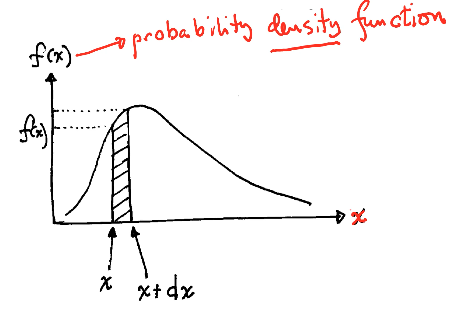
\includegraphics[width=0.9\linewidth]{st2131-pdf.png} 
  \end{minipage}
  \begin{minipage}[c]{0.55\linewidth}
    \begin{align*}
      P(x < X < x + \dx) &= \int^{x+\dx}_x f(y) \mathop{dy} 
                      \\ &\approx f(x) \cdot \dx
    \end{align*}

    pdf at $x$, $f(x) \approx \frac{P(x < X < x + \dx)}{\dx}$
  \end{minipage}

  \textbf{N6} - if $X$ is a continuous r.v. with pdf $f(x)$ and cdf $F(x)$, then $f(x) = \frac{d}{\dx}F(x)$. (\textit{Fundamental Theorem of Calculus})

  \textbf{N7} - median of $X$, $x$ occurs where $F(x) = \frac{1}{2}$ 

  \subsection{Generating a Uniform r.v.}

  if $X$ is a continuous r.v. with cdf $F(x)$, then 

  \begin{itemize}
    \item \textbf{N8} - $F(X) = U \sim uniform(0, 1)$.

      \begin{niceproof}
        let $Y = F(X)$. then cdf of $Y$, $F_Y(y)$ = $P(Y \leq y) = P(F(X) \leq y) = P(X \leq F^{-1}(y)) = F(F^{-1}(y)) = y $.
      \end{niceproof}

    \item \textbf{N9} - $X = F^{-1}(U) \sim$ cdf $F(x)$.
      \begin{itemize}
        \item generating a r.v. from a uniform(0, 1) r.v. and a r.v. with cdf $F(x)$.
      \end{itemize}
  \end{itemize}

  \subsection{Uniform Random Variable}

  $X$ is a \ildefinition{uniform r.v.} on the interval $(\alpha, \beta)$, $X \sim Uniform(\alpha, \beta)$ 

  if its pdf is given by 

  \begin{minipage}[c]{0.25\linewidth}
    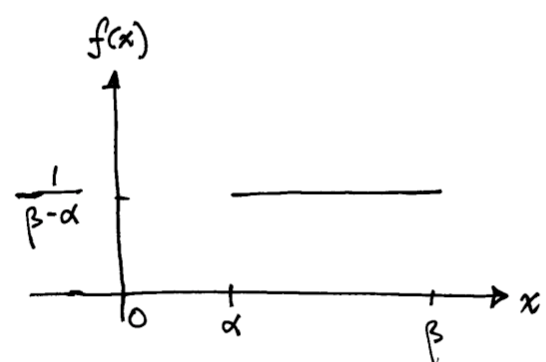
\includegraphics[width=0.95\linewidth]{st2131-uniform-rv.png} 
  \end{minipage}
  \begin{minipage}[c]{0.7\linewidth}
    \begin{tightcenter}
      $f(x) = \begin{cases} \frac{1}{\beta-\alpha}, &\alpha<x<\beta \\ 0, &\text{otherwise} \end{cases}$

      $E(X) = \frac{\alpha + \beta}{2}, \quad Var(X) = \frac{(\beta - \alpha)^2}{12}$
    \end{tightcenter}
  \end{minipage}

  if $X \sim Uniform(\alpha, \beta)$, then $\frac{x - \alpha}{\beta - \alpha} \sim Uniform (0,1)$
  \subsection{Normal Random Variable}

  $X$ is a \ildefinition{normal r.v.} with parameters $\mu$ and $\sigma^2$, $X \sim N(\mu,\sigma^2)$ 

  if the pdf of $X$ is given by

  \begin{tightcenter}
    $f(x) = \frac{1}{\sqrt{2\pi} \sigma}e^{-\frac{1}{2} (\frac{x}{\mu}\sigma)^2}$, $\quad -\infty < x < \infty$

    $E(x) = \mu, \quad Var(X) = \sigma^2$
  \end{tightcenter}

  \begin{minipage}[c]{0.3\linewidth}
    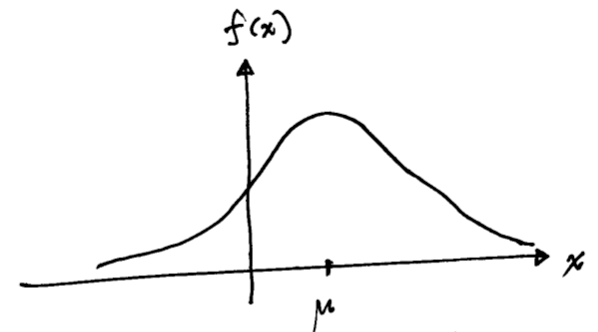
\includegraphics[width=0.9\linewidth]{st2131-normal-distribution.png} 
  \end{minipage}
  \begin{minipage}[c]{0.67\linewidth}
    if $X \sim N(\mu, \sigma^2)$, then $\frac{X - \mu}{\sigma} \sim N(0, 1)$

    if $Y \sim N(\mu, \sigma^2)$ and $a$ is a constant, $F_y(a) = \Phi (\frac{a-\mu}{\sigma}) $
  \end{minipage}

  \definition{standard normal distribution} $X \sim N(0,1)$

  \begin{itemize}
    \item $F(x) = P(X \leq x) = \frac{1}{\sqrt{r \pi}} \int^x_{-\infty} e^{-\frac{1}{2}y^2} \mathop{dy} = \Phi(x)$
  \end{itemize}

  \subsubsection{Normal Approximation to the Binomial Distribution}

  \begin{tightcenter}
    if $S_n \sim Binomial(n, p)$, then $\frac{S_n - np}{\sqrt{np(1-p)}} \sim N(0,1)$ for large $n$.

    $\mu = np$, $\quad \sigma^2 = np(1-p)$
  \end{tightcenter}

  \subsection{Exponential Random Variable}

  a \textit{continuous} r.v. $X$ is a \ildefinition{exponential r.v.}, $\quad X \sim Exponential(\lambda)$ or $Exp(\lambda)$ 

  if for some $\lambda > 0$, its pdf is given by 

  \begin{minipage}[c]{0.3\linewidth}
    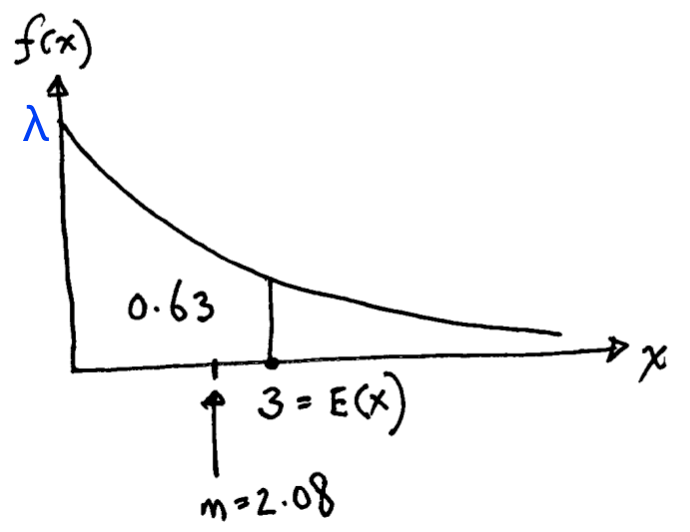
\includegraphics[width=0.95\linewidth]{st2131-exponential-rv-example.png} 
  \end{minipage}
  \begin{minipage}[c]{0.65\linewidth}
    \begin{tightcenter}
      $f(x) = \begin{cases} \lambda e^{-\lambda x}, &x \geq 0 \\ 0, &\text{otherwise} \end{cases}$

      $E(X) = \frac{1}{\lambda}, \quad Var(X) = \frac{1}{\lambda^2}$
      \ \\ \ 

      $P(X < a) = \int^a_0 \lambda e^{-\lambda x} \dx$
    \end{tightcenter}
  \end{minipage}

  \begin{itemize}
    \item an exponential r.v. is \textit{memoryless}.
      \begin{itemize}
        \item a non-negative r.v. is \definition{memoryless} if $P(X > s + t \mid X > t) = P(X > s)$ for all  $s, t > 0$.
      \end{itemize}
  \end{itemize}

  \subsection{Gamma Distribution}

  a r.v. $X$ has a \ildefinition{gamma distribution}, $\quad X \sim Gamma(\alpha, \lambda)$ 

  with parameters $(\alpha, \lambda)$, $\lambda > 0$ and $\alpha > 0$ if its pdf is given by 

  \begin{tightcenter}
    $f(x) \begin{cases} \frac{\lambda e^{-\lambda x}(\lambda x)^{\alpha - 1}}{\Gamma(\alpha)} , &x \geq 0 \\ 0, &x < 0 \end{cases} $

    $E(X) = \frac{\alpha}{\lambda} \quad Var(X) = \frac{\alpha}{\lambda^2}$
  \end{tightcenter}

  where the gamma function $\Gamma(\alpha)$ is defined as 
  $\Gamma (\alpha) = \int^\infty_0 e^{-y} y^{\alpha - 1} \mathop{dy} $.

  \begin{minipage}[c]{0.4\linewidth}
    \begin{tightcenter}
      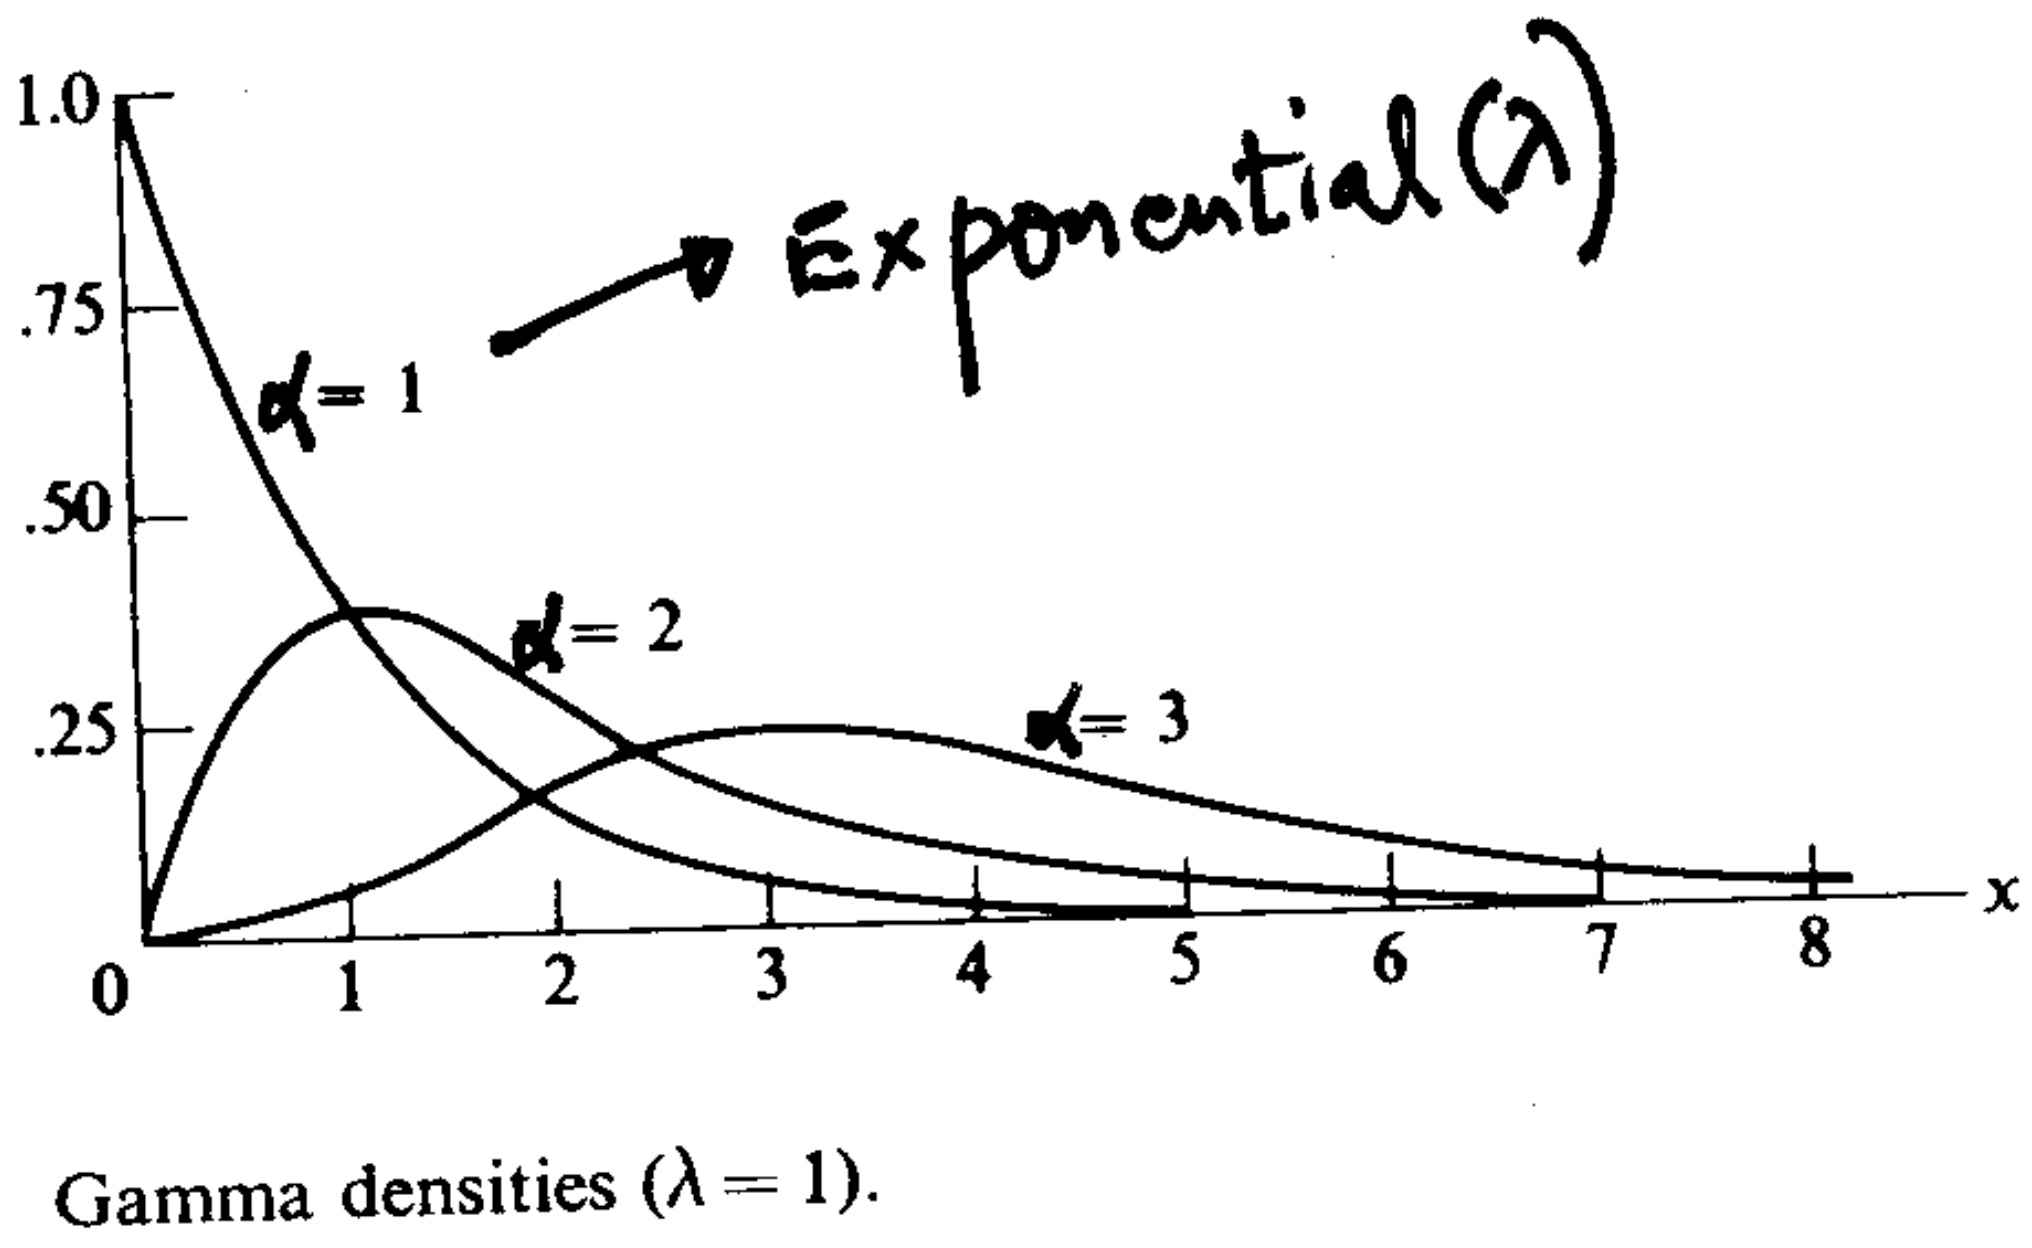
\includegraphics[width=0.9\linewidth]{st2131-gamma-distribution.png} 
    \end{tightcenter}
  \end{minipage}
  \begin{minipage}[c]{0.55\linewidth}
    \textbf{N1} - $\Gamma(\alpha) = (\alpha - 1) \Gamma(\alpha-1) $
    \begin{niceproof}
      using integration by parts of LHS to RHS
    \end{niceproof}

    \textbf{N2} - if $\alpha$ is an integer $n$, then $\Gamma(n) = (n-1)!$

    \textbf{N3} - if $X \sim Gamma(\alpha, \lambda)$ and $\alpha = 1$, then $X \sim Exp(\lambda)$.
  \end{minipage}

  \textbf{N4} - for events occurring randomly in time following the 3 assumptions of poisson distribution, 
  the \textbf{amount of time elapsed} until a total of $n$ events has occurred is a gamma r.v. with parameters $(n, \lambda)$.
  \begin{itemize}
    \item time at which the $n$-th event occurs, $T_n \sim Gamma(n, \lambda)$ 
    \item number of events in time period $[0, t]$, $N(t) \sim Poisson(\lambda t)$
  \end{itemize}

  \textbf{N5} - $Gamma(\alpha = \frac{n}{2}, \lambda = \frac{1}{2}) = \chi^2_n \quad$ (chi-square distribution to $n$ degrees of freedom)


  \subsection{Beta Distribution}

  a r.v. $X$ is said to have a \ildefinition{beta distribution}, $X \sim Beta(a, b)$ 

  \begin{tightcenter}
    $f(x) = \begin{cases} \frac{1}{\beta(a, b)} x^{a-1} (1-x)^{b-1}, &0 < x < 1 \\ 0, &\text{otherwise} \end{cases} $

    $E(X) = \frac{a}{a+b} \quad Var(X) = \frac{ab}{(a+b)^2 (a+b+1)} $
  \end{tightcenter}

  \begin{tightcenter}
    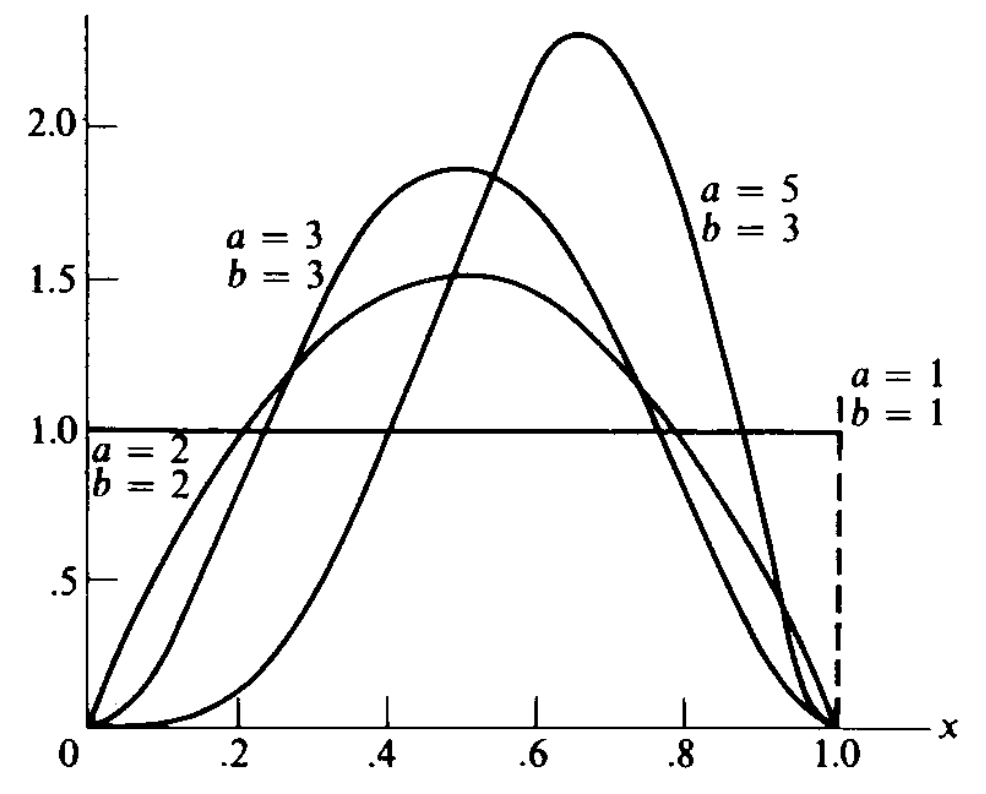
\includegraphics[width=0.35\linewidth]{st2131-beta-distribution-2.png} 
    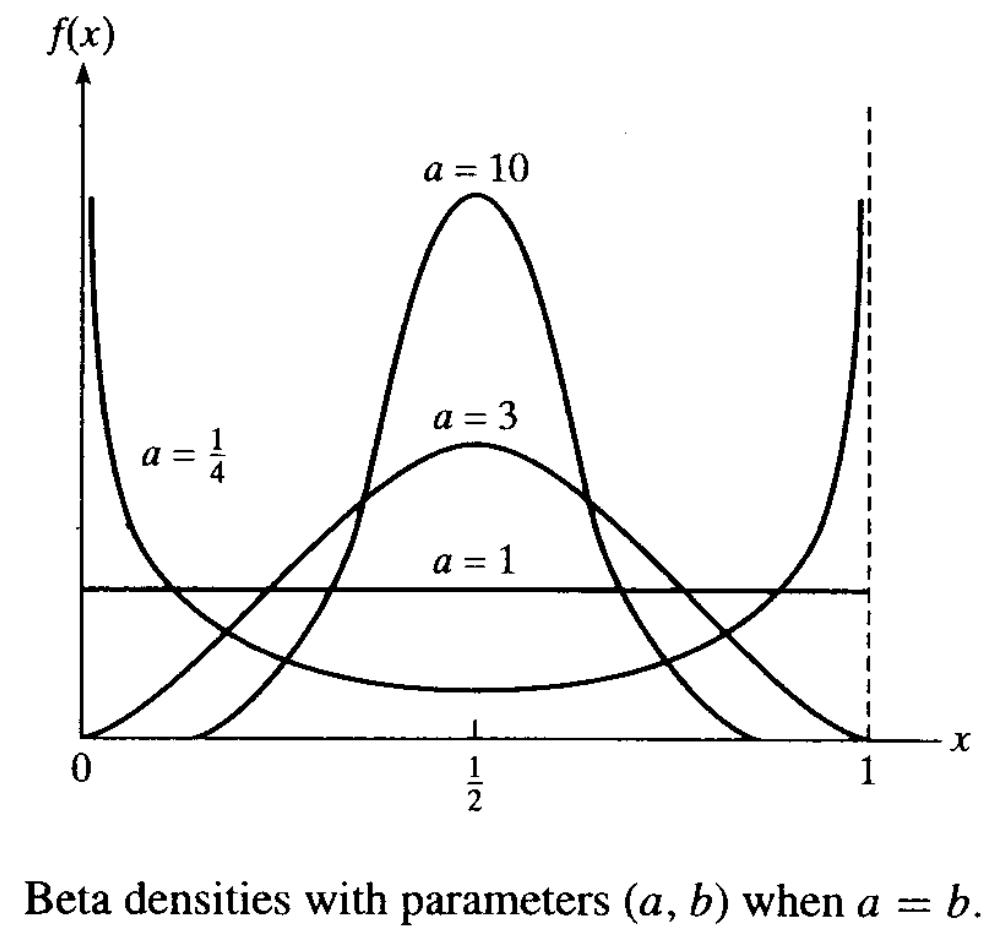
\includegraphics[width=0.35\linewidth]{st2131-beta-distribution-1.png} 
  \end{tightcenter}

  \textbf{N1} - $\beta(a, b) = \int^1_0 x^{a-1}(1-x)^{b-1} \dx$

  \textbf{N2} - $\beta(a=1, b=1) = Uniform(0, 1)$

  \textbf{N3} - $\beta(a, b) = \frac{\Gamma(a) \Gamma(b)}{\Gamma(a+b)}$


  \subsection{Cauchy Distribution}

  a r.v. $X$ has a cauchy distribution, $\quad X \sim Cauchy(\theta)$ 

  with parameter $\theta$, $\-\infty < \theta < \infty$ if its density is given by 

  \begin{tightcenter}
    $f(x) = \frac{1}{\pi} \cdot \frac{1}{1 + (x-\theta)^2} $, $-\infty < x < \infty$
  \end{tightcenter}


  \section{06. JOINTLY DISTRIBUTED RANDOM VARIABLES}

  \subsection{Joint Distribution Function}

  \begin{tightcenter}
    the \ildefinition{joint cumulative distribution function} of the pair of r.v. $X$ and $Y$ is $\rightarrow$
    $F(x, y) = P(X \leq x, Y \leq y)$,  $-\infty < x < \infty$, $\; -\infty < y < \infty$
  \end{tightcenter}

  \textbf{N1} - \ildefinition{marginal cdf of $X$}, $F_X(x) = \lim\limits_{y \to \infty} F(x, y)$.

  \textbf{N2} - \ildefinition{marginal cdf of $Y$}, $F_Y(y) = \lim\limits_{x \to \infty} F(x, y)$.

  \begin{minipage}[c]{0.25\linewidth}
    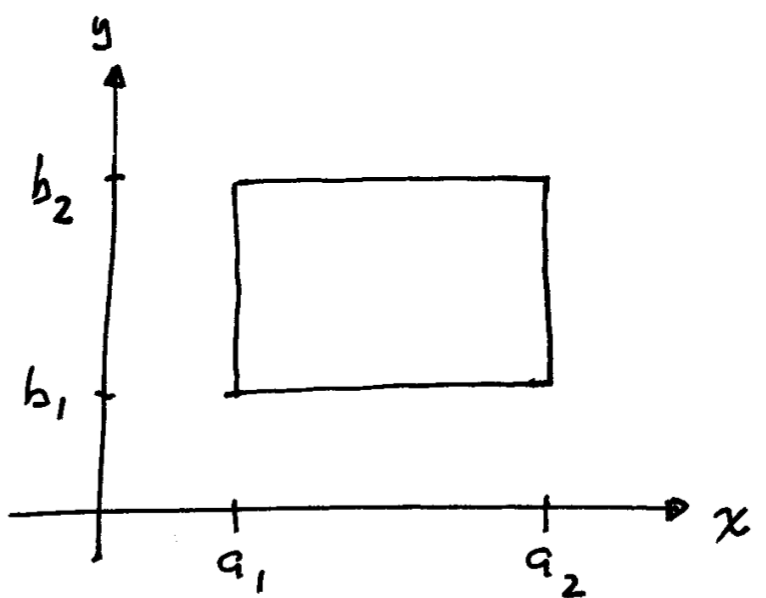
\includegraphics[width=0.95\linewidth]{st2131-joint-distribution-summation.png} 
  \end{minipage}
  \begin{minipage}[c]{0.72\linewidth}
    \textbf{N3} - $P(X > a, Y > b) = 1 - F_X(a) - F_Y(b) + F(a, b) $

    \textbf{N4} - $P(a_1 < X \leq a_2, b_1 < Y \leq b_2)$
    \\* $\quad \quad = F(a_2, b_2) + F(a_1, b_1) - F(a_1, b_2) - F(a_2, b_1) $
  \end{minipage}

  \subsection{Joint Probability Mass Function}

  \begin{tightcenter}
    if $X$ and $Y$ are both discrete r.v., then their \ildefinition{joint pmf} is defined by

    $p(i, j) = P(X=i, Y=j)$
  \end{tightcenter}

  \textbf{N1} - \ildefinition{marginal pmf of $X$}, $P(X=i) = \sum_j P(X=i, Y=j)$ 

  \textbf{N2} - \ildefinition{marginal pmf of $Y$}, $P(Y=i) = \sum_i P(X=i, Y=j)$ 

  \subsection{Joint Probability Density Function}

  the r.v. $X$ and $Y$ are said to be \textit{jointly continuous} if there is a function $f(x,y)$ called the \ildefinition{joint pdf}, such that for any two-dimensional set $C$, 

  \begin{tightcenter}
    $P[(X, Y) \in C] = \iint\limits_C f(x, y) \dx \mathop{dy}$

    $= $ volume under the surface over the region $C$.
  \end{tightcenter} 

  \begin{minipage}[c]{0.4\linewidth}
    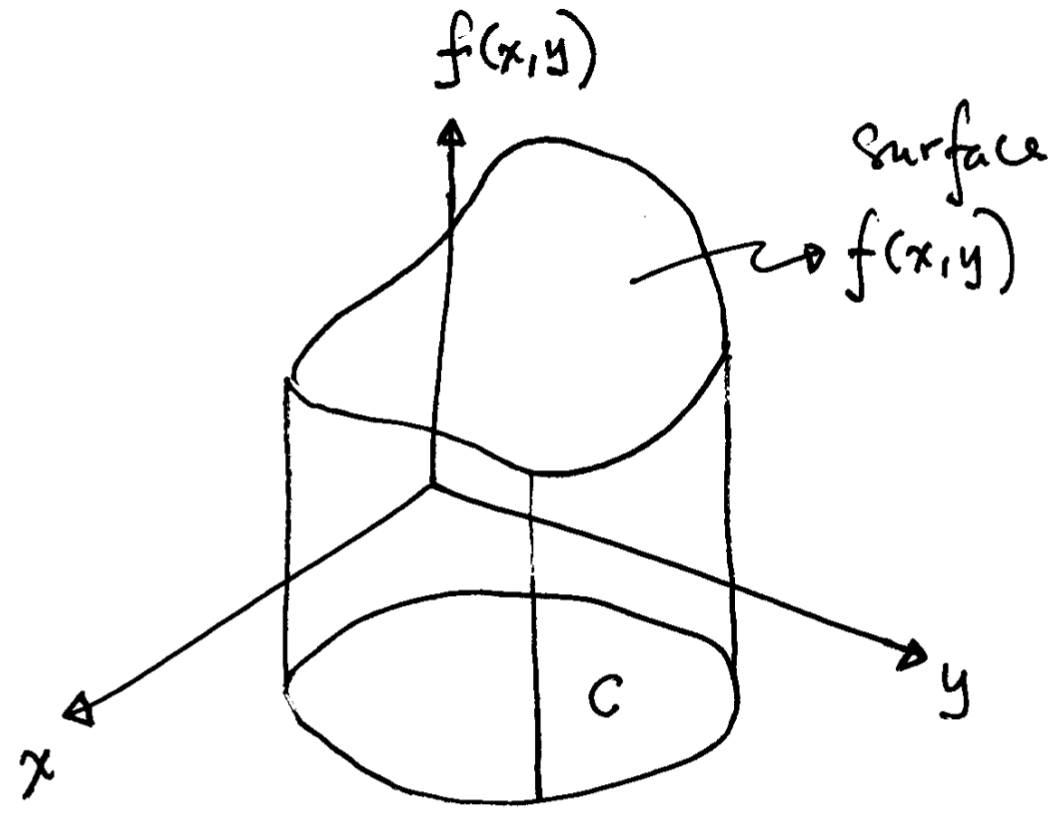
\includegraphics[width=0.9\linewidth]{st2131-joint-pmf-geometric.png}
  \end{minipage}
  \begin{minipage}[c]{0.55\linewidth}
    \textbf{N1} - if $C = \{(x, y): x \in A, y \in B \}$, then 
    $P(X \in A, Y \in B) = \int\limits_B \int\limits_A f(x, y) \dx \dy$

    \textbf{N2} - $F(a, b)$
    \\* $\quad = P\Big(X \in (-\infty, a], Y \in (-\infty, b]\Big)$
    \\* $\quad = \int^b_{-\infty} \int^a_{-\infty} f(x, y) \dx \dy $

    \ \\
    \textbf{N3} - $f(a, b) = \frac{\delta^2}{\delta a \delta b} F(a, b)$
  \end{minipage}

  \subsubsection{interpretation of pdf}

  \begin{minipage}[c]{0.3\linewidth}
    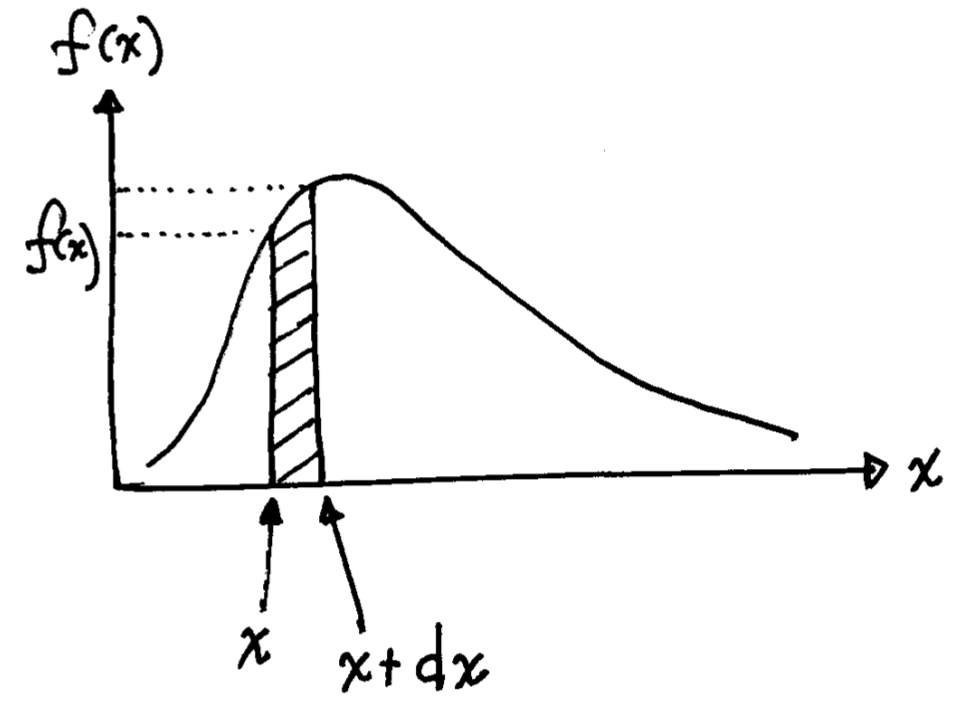
\includegraphics[width=0.95\linewidth]{st2131-pdf-interpretation.png} 
  \end{minipage}
  \begin{minipage}[c]{0.65\linewidth}
    \begin{align*}
      P(x < X < x + \dx) &= \int^{x + \dx}_x f(y) \dy \\ &\approx f(x) \dx  
    \end{align*}

    \ 
    \begin{tightcenter}
      pdf at $x$, $f(x) \approx \frac{P(x < X < x + \dx)}{\dx}$
    \end{tightcenter}
  \end{minipage}

  \subsubsection{interpretation of joint pdf}

  \begin{minipage}[c]{0.3\linewidth}
    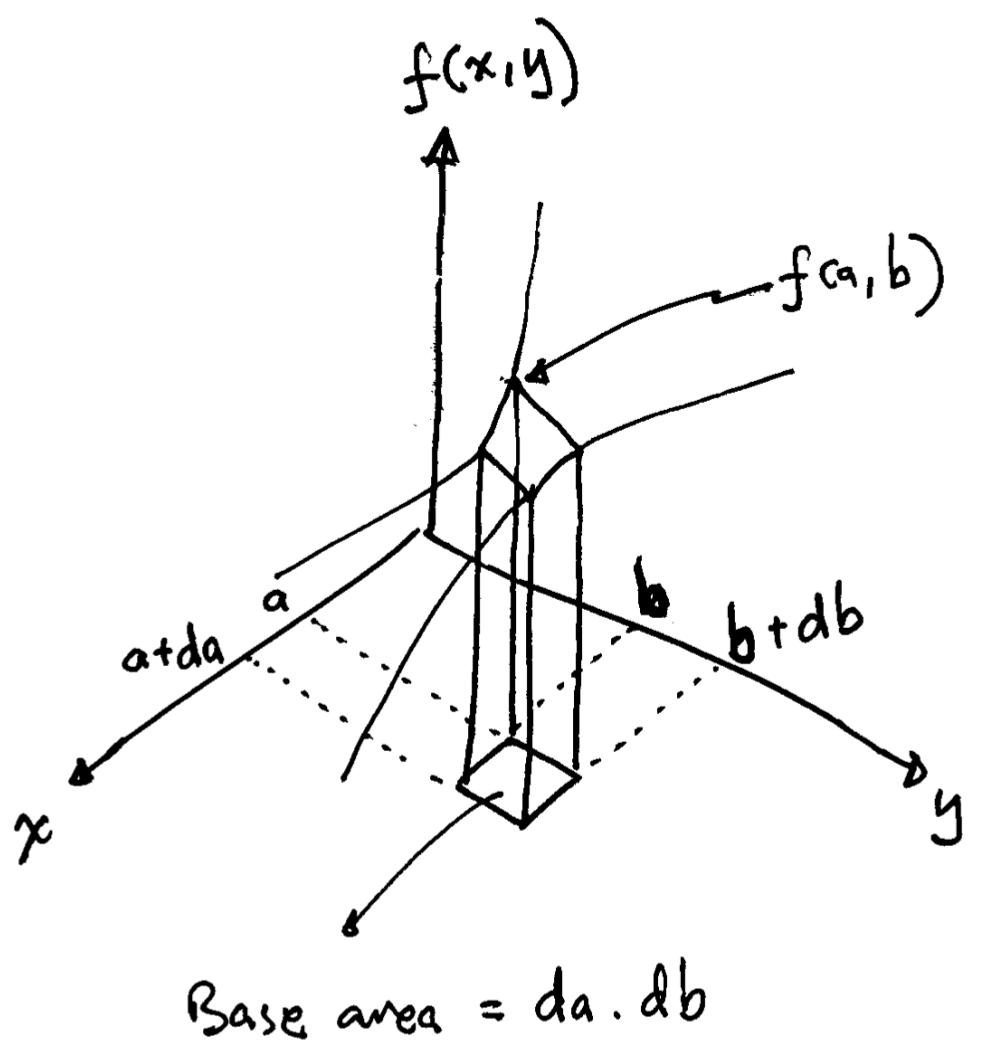
\includegraphics[width=0.95\linewidth]{st2131-joint-pdf-interpretation.png} 
  \end{minipage}
  \begin{minipage}[c]{0.65\linewidth}
    $P(a < X < a + \mathop{da}, b < Y < b + \mathop{db})$
    \\* $\quad = \int^{b + db}_b \int^{a + da}_a f(x, y) \dx \dy$
    \\* $\quad \approx f(a, b) \mathop{da}\mathop{db} \quad\quad$ (density of probability)

    \ildefinition{marginal pdf of $X$}, $f_X(x) = \int^\infty_{-\infty} f(x, y) \dy$

    \ildefinition{marginal pdf of $Y$}, $f_Y(x) = \int^\infty_{-\infty} f(x, y) \dx$
  \end{minipage}

  \subsubsection{how to do a double integral}

  \begin{minipage}[c]{0.55\linewidth}
    \textbf{example} - given the joint pdf of $X$ and $Y$, find the pdf of r.v. $X/Y$.

    \begin{niceproof}[ans]
      set dummy variable $W = X/Y$, 
      then $F_W(w) = P(W \leq w) = P(\frac{X}{Y} \leq w)$

      $P(\frac{X}{Y} \leq w) = \int^\infty_0 \int^{wy}_0 e^{-x-y} \dx \dy $
    \end{niceproof}
  \end{minipage}
  \begin{minipage}[c]{0.4\linewidth}
    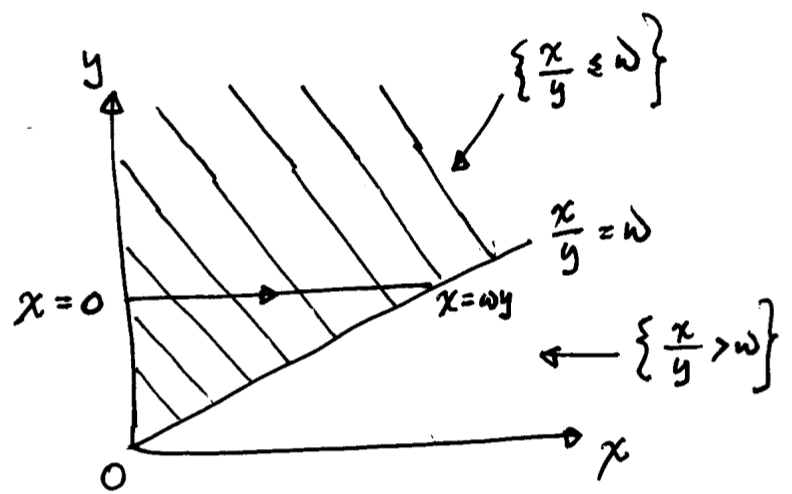
\includegraphics[width=0.95\linewidth]{st2131-double-integral-eg-3.png} 
  \end{minipage}


  \subsection{Independent Random Variables}

  \textbf{N1} - $X$, $Y$ are \definition{independent} $P(X \in A, Y \in B) = P(X \in A) \cdot P(Y \in B)$

  \textbf{N2} - $X$ and $Y$ are \definition{independent} $P(X \leq a, Y \leq b) = P(X \leq a) \cdot P(Y \leq b) $
  \\* $\quad$ or $F(a, b) = F_X(a) \cdot F_Y(b)$ $\quad \Rightarrow $ joint cdf is the product of the marginal cdfs

  \textbf{N3} - \textit{discrete case}: discrete r.v. $X$ and $Y$ are \ildefinition{independent} $\iff$
  \begin{tightcenter}
    $P(X=x, Y=y) = P(X=x) \cdot P(Y=y)$ for all $x, y$.
  \end{tightcenter}

  \textbf{N4} - \textit{continuous case}: jointly continuous r.v. $X$ and $Y$ are \ildefinition{independent} $\iff$
  \begin{tightcenter}
    $f(x, y) = f_X(x) \cdot f_Y(y)$ for all $x, y$.

    $-\infty < x < \infty,\quad -\infty < y < \infty$
  \end{tightcenter}

  \textbf{N5} - independence is a \definition[relation]{symmetric} $X$ indep of $Y$ $\iff$ $Y$ indep of $X$

  \begin{tightcenter}
    if $X$ and $Y$ are independent, then for any functions $h$ and $g$, 
    \\* $E[ g(X) h(Y) ] = E[g(X)] \cdot E[h(Y)] $
  \end{tightcenter}

  \subsection{Sum of Independent Random Variables}

  \textbf{N1} - for independent, continuous r.v. $X$ and $Y$ having pdf $f_X$ and $f_Y$, 
  \begin{tightcenter}
    $F_{X+Y}(a) = \int^\infty_{-\infty} F_X (a-y) f_Y(y) \dy $

    $f_{X+Y}(a) = \int^\infty_{-\infty} f_X (a-y) f_Y(y) \dy $
  \end{tightcenter}

  \subsubsection{Distribution of Sums of Independent r.v.}

  for $i = 1, 2, \dots, n$, 

  \begin{enumerate}
    \item $X_i \sim Gamma(t_i, \lambda) \quad\Rightarrow\quad \sum\limits^n_{i=1} X_i \sim Gamma(\sum\limits^n_{i=1} t_i, \lambda)$
    \item $X_i \sim Exp(\lambda) \quad\Rightarrow\quad \sum\limits^n_{i=1}X_i \sim Gamma(n, \lambda)$
    \item  $Z_i \sim N(0, 1) \quad\Rightarrow\quad \sum\limits^n_{i=1} z^2_i \sim \chi^2_n = Gamma(\frac{n}{2}, \frac{1}{2}) $
    \item $X_i \sim N(\mu_i, \sigma_i^2) \quad\Rightarrow\quad \sum\limits^n_{i=1}X_i \sim N( \sum\limits^n_{i=1} \mu_i, \sum\limits^n_{i=1} \sigma^2_i ) $
    \item $X \sim Poisson(\lambda_1), Y \sim Poisson (\lambda_2) \Rightarrow X+Y \sim Poisson(\lambda_1 + \lambda_2)$
    \item $X \sim Binom(n, p), Y \sim Binom(m, p) \Rightarrow X+Y \sim Binom(n+m, p) $
  \end{enumerate}

  \subsubsection{Conditional Distribution (discrete)}

  for discrete r.v. $X$ and $Y$, the \ildefinition{conditional pmf} of  $X$ given that $Y=y$ is
  \begin{tightcenter}
    $P_{X \vert Y} (x \vert y) = P(X = x \vert Y = y) = \frac{P(X = x, Y = y)}{P(Y = y)} = \frac{p(x, y)}{p_Y(y)} $
  \end{tightcenter}

  for discrete r.v. $X$ and $Y$, the \ildefinition{conditional pdf} of  $X$ given that $Y=y$ is
  \begin{tightcenter}
    $F_{X \vert Y} (x \vert y) = P(X \leq x \vert Y = y) = \sum\limits_{a \leq x}P(X = a, Y = y) = \sum\limits_{a \leq x} P_{X \vert Y} (a \vert y) $
  \end{tightcenter}

  \textbf{N0} - equivalent notation: 
  \begin{itemize}
    \item $P_{X \vert Y}(x \vert y) = P(X = x \vert Y = y)$
    \item $P_X(x) = P(X = x)$
  \end{itemize}

  \textbf{N1} - if $X$ is independent of $Y$, then $P_{X \vert Y}(x \vert y) = P_X(x)$

  \subsubsection{Conditional Distribution (continuous)}

  for $X$ and $Y$ with joint pdf $f(x, y)$, the \ildefinition{conditional pdf} of $X$ given that $Y = y$ is
  \begin{tightcenter}
    $f_{X \vert Y} (x \vert y) = \frac{f(x, y)}{f_Y(y)} \quad$ for all $y$ s.t. $f_Y(y) > 0$

    $F_{X \vert Y} (a \vert y) = P(X \leq a \vert Y = y) = \int\limits^a_{-\infty} f_{X \vert Y} (x \vert y) \dx $ 
  \end{tightcenter}

  \textbf{N1} - for any set $A$, $P(X \in A \vert Y = y) = \int\limits_A f_{X \vert Y} (x \vert y) \dy$

  \textbf{N2} - if $X$ is independent of $Y$, then $f_{X \vert Y} (x \vert y) = f_X (x)$.

  \attention "find the marginal/conditional pdf of $Y$" $\Rightarrow$ must include the \textbf{range} too!! 


  \subsection{Joint Probability Distribution of Functions of r.v.}

  Let $X_1$ and $X_2$ be jointly continuous r.v. with joint pdf $f_{x_1, x_2} (x_1, x_2)$. 
  Suppose $Y_1 = g_1 (X_1, X_2)$ and $Y_2 = g_2 (X_1, X_2)$ satisfy

  \begin{enumerate}
    \item the equations $y_1 = g_1 (X_1, X_2)$ and $y_2 = g_2 (X_1, X_2)$ can be \textit{uniquely} solved for $x_1$, $x_2$ in terms of $y_1$ and $y_2$
    \item $g_1(x_1, x_2)$ and $g_2(x_1, x_2)$ have continuous partial derivatives at all points $(x_1, x_2)$ 
      such that $J(x_1, x_2) = \left\vert \begin{smallmatrix} \frac{\delta g_1}{\delta x_1} & \frac{\delta g_1}{\delta x_2}
      \\ \frac{\delta g_2}{\delta x_1} & \frac{\delta g_2}{\delta x_2} \end{smallmatrix} \right\vert = \frac{\delta g_1}{\delta x_1} \cdot \frac{\delta g_2}{\delta x_2} - \frac{\delta g_2}{\delta x_1} \cdot \frac{\delta g_1}{\delta x_2} \neq 0 $
    \end{enumerate}

    then 
    \begin{tightcenter}
      $f_{Y_1, Y_2} (y_1, y_2) = f_{X_1, X_2} (x_1, x_2) \frac{1}{\abs{J(x_1, x_2)}} $

      where $x_1 = h_1(y_1, y_2), x_2 = h_2(y_1, y_2)$
    \end{tightcenter}


    \section{07. PROPERTIES OF EXPECTATION}

    \begin{itemize}
      \item for a \textbf{discrete} r.v. $X$, $E(X) = \sum_x x \cdot p(x) = \sum_x \cdot P(X = x)$
      \item for a \textbf{continuous} r.v. $X$, $E(X) = \int^\infty_{-\infty} x \cdot f(x) \dx$
      \item for a \textbf{non-negative integer-valued} r.v. $Y$, $E(Y) = \sum^\infty_{i=1} P(Y \geq i)$
      \item for a \textbf{non-negative} r.v. $Y$, $E(Y) = \int^\infty_{-\infty} P(Y > y)\dy$
    \end{itemize}

    \subsection{Expectations of Sums of Random Variables}

    \begin{tightcenter}
      for $X$ and $Y$ with joint pmf $p(x, y)$ and joint pdf  $f(x, y)$, 

      $E[g(x, y)] = \sum\limits_y \sum\limits_x g(x, y) p(x, y)$

      $ E[g(x, y)] = \int^\infty_{-\infty} \int^\infty_{-\infty} g(x, y) f(x, y) \dx \dy $
    \end{tightcenter}

    \textbf{N2} - if $P(a \leq X \leq b) = 1$, then $a \leq E(X) \leq b$

    \textbf{N4} - for r.v.s $X$ and $Y$, if $X \geq Y$, then $E(X) \geq E(Y)$

    \textbf{N5} - let $X_1, \dots, X_n$ be independent and identically distributed r.v.s having distribution $P(X_i \leq x) = F(x)$ and expected value $E(X_i) = \mu$. 
    \begin{tightcenter}
      if $\bar{X} = \sum\limits^n_{i=1} \frac{X_i}{n}$, then $E(\bar{X}) = \mu$
    \end{tightcenter}

    \textbf{N6} - $\bar{X}$ is the \ildefinition{sample mean}.
    $\quad\quad\Rightarrow$ sample mean = population mean

    \attention trick: express a r.v. as a sum of r.v. with easier to find expectation

    \subsubsection{examples}

    \begin{itemize}
      \item hypergeometric with $r$ red balls out of  $N$ balls  with $n$ trials
        \begin{itemize}
          \item indicator r.v. $=1$ if the $i$th ball selected is red \item $P(Y_i = 1) = \frac{r}{N} \Rightarrow E(Y_i) = \frac{r}{N} \Rightarrow E(X) = \sum^n_{i=1}Y_i = n\frac{r}{N} $
        \end{itemize}
      \item coupon collector problem: 
        \begin{itemize}
          \item let $X$ = number of coupons collected for a complete set
          \item let $X_i$ = additional number to be collected to obtain distinct type after $i$ distinct types have been collected.  $X_i \sim Geometric(p = \frac{N-i}{N} )$
          \item $E(X) = \sum^{N-1}_{i=1} E(X_i) = 1 + \frac{1}{\frac{N-1}{N}} + \frac{1}{\frac{N-2}{N}} + \dots + \frac{1}{\frac{1}{N}}$ 
            \\* $ \quad = N(\frac{1}{N} + \frac{1}{N-1} + \dots + 1) $
        \end{itemize}
    \end{itemize}

    \subsection{Covariance, Variance of Sums and Correlations}

    \definition{covariance} measure of \textit{linear relationship}

    \begin{tightcenter}
      $Cov (X, Y) = E[ (X-E[X]) (Y - E[Y]) ] $
      \\* $Cov(X, Y) = E(XY) - E(X)E(Y)$
    \end{tightcenter}

    \textbf{N1} - $X$ and $Y$ are independent $\Rightarrow Cov(X, Y) = 0$

    \textbf{N2} - $Cov(X, Y) = 0 \not\Rightarrow$ $X$ and $Y$ are independent. 
    \textit{Proof.}
    let $E(X) = 0$, $E(XY) = 0 \Rightarrow Cov(X, Y) = 0$, but not independent
    e.g. non-linear relationship

    \subsubsection{Covariance properties}

    \begin{enumerate}
      \item $Cov(X, Y) = Cov(Y, X)$ 
      \item $Cov(X, X) = Var(X)$ 
      \item $Cov(aX, Y) = aCov(X, Y)$
      \item $Cov (\sum\limits^n_{i=1} X_i, \sum\limits^m_{j=1} Y_j) = \sum\limits^n_{i=1} \sum\limits^m_{j-1} Cov(X_i, Y_j) $
      \item $Cov (I_A, I_B) = P(B) [ P(A \vert B) - P(A) ] $
    \end{enumerate}

    for variance:

    \textbf{N1} - $Var (\sum\limits^n_{i=1} X_i) = \sum\limits^n_{i=1} Var(X_i) + 2 \mathop{\sum\sum}\limits_{i<j} Cov(X_i, X_j) $

    \textbf{N2} - if $X_1, \dots, X_n$ are \textit{pairwise independent}, $Var(\sum\limits^n_{i=1} X_i) = \sum\limits^n_{i=1} Var(X_i)$

    \textbf{N3} - for $n$ independent and identically distributed r.v. with variance  $\sigma^2$, 
    \begin{tightcenter}
      $\bar{X} = \frac{1}{n} \sum\limits^n_{i=1} x_i \quad\quad S^2 = \frac{1}{n-1} \sum\limits^n_{i=1} (x_i - \bar{x})^2$ 

      $Var (\bar{X}) = \frac{\sigma^2}{n} \quad\quad E(S^2) = \sigma^2 \quad\quad\quad\quad$
    \end{tightcenter}
    $\Rightarrow$ $S^2$ is an \textit{unbiased estimator} for $\sigma^2$.

    \subsubsection{Correlation}

    \begin{tightcenter}
      \ildefinition{correlation} of two r.v. $X$ and $Y$, 
      $\rho(X, Y) = \frac{Cov(X, Y)}{\sqrt{Var(X) \cdot Var(Y)}}$
    \end{tightcenter}

    \textbf{N1} - $-1 \leq \rho(X, Y) \leq 1$
    where  $-1$ and $1$ denote a perfect negative and positive linear relationship respectively.

    \textbf{N2} - $\rho(X, Y) = 0 \Rightarrow$ no \textit{linear} relationship - uncorrelated

    \textbf{N3} - $\rho(X, Y) = 1 \Rightarrow Y = aX + b, a = \frac{\delta y}{\delta x} > 0$

    \textbf{N4} - for independent events $A$, $B$ with indicator r.v. $I_A$, $I_B$: $Cov(I_A, I_B) = 0$. 

    \textbf{N5} - deviation is not correlated with the sample mean. For independent \& identically distributed r.v. $X_1, X_2, \dots, X_n$ with variance $\sigma^2$, then $Cov(X_i - \bar{X}, \bar{X}) = 0$.

    \subsection{Conditional Expectation}

    the \ildefinition{conditional expectation} of $X$ given that $Y=y$, $\quad \forall y$ s.t. $P_Y(y) > 0$, is:

    \begin{tightcenter}
      $E[X \vert Y=y] = \sum\limits_x x \cdot P(X=x \vert Y=y) = \sum\limits_x x \cdot p_{X \vert Y} (x \vert y)$

      $E(X \vert Y=y) = \int\limits^\infty_{-\infty} x \cdot f_{X \vert Y}(x \vert y) \dx = \int\limits^\infty_{-\infty} x \cdot \frac{f(x, y)}{f_Y(y)} \dx$

      \attention note the range for $f_{X \vert Y}(x \vert y)$
    \end{tightcenter}

    \textbf{N1} - If $X, Y \sim Geometric(p)$, 
    \\* then $P(X=i \vert X+Y=n) = \frac{1}{n-1}$, a uniform distribution.

    \textbf{N2} - $E(X \vert X+Y=n) = \sum^{n-1}_{i=1} i \cdot P(X=i \vert X+Y=n) = \frac{n}{2}$

    \begin{tightcenter}
      discrete case: $E[g(x) \vert Y=y] = \sum\limits_x g(x) P_{X \vert Y} (x \vert y)$

      continuous case: $E[g(x) \vert Y=y] = \int^\infty_{-\infty} g(x) f_{X \vert Y} (x \vert y) \dx$

      then $E(X) = E_{ \text{w.r.t. } y} (E_{ \text{w.r.t. } X \vert Y=y}(X \vert Y)) $
    \end{tightcenter}

    \subsubsection{Deriving Expectation}

    $E(X) = E_Y(E_X(X \vert Y))$

    \begin{tightcenter}
      discrete case: $E(X) = \sum\limits_y E(X \vert Y=y) P(Y=y)$

      continuous case: $E(X) = \int^\infty_{-\infty} E(X \vert Y=y)f_Y(y) \dy$
    \end{tightcenter}

    \textbf{N3} - 3 methods for finding $E(X)$ given $f(x, y)$
    \begin{enumerate}
      \item using $E(g(x, y)) = \int^\infty_{-\infty} \int^\infty_{-\infty} g(x, y) f(x, y) \dx \dy$ $\quad \Rightarrow$ let $g(x, y) = x$
      \item using $E(X) = \int^\infty_{-\infty} x f_X(x) \dx$
      \item using $E(X) = \int^\infty_{-\infty} E(X \vert Y=y) f_Y(y) \dy$
    \end{enumerate}

    \textbf{N4} - $E(\sum\limits^N_{i=1} X_i) = E_N(E(\sum\limits^N_{i=1} X_i \vert N)) = \sum\limits^\infty_{n=0} E(\sum\limits^N_{i=1} X_i \vert N=n) \cdot P(N=n) $


    \subsubsection{Computing Probabilities by Conditioning}

    \begin{tightcenter}
      \textit{discrete}: $\quad P(E) = \sum\limits_y P(E \vert Y=y) P(Y=y)$ 

      \textit{continuous}: $\quad P(E) = \int\limits^\infty_{-\infty} P(E \vert Y=y) f_Y(y) \dy$ 
    \end{tightcenter}

    \begin{niceproof}
      $X$ is an indicator r.v.;
      $E(X | Y=y) = P(X=1 \vert Y=y) = P(E \vert Y=y)$
    \end{niceproof}

    \textbf{N5} - $P(X < Y) = \int P(X < Y \vert Y = y) \cdot f_Y(y)$

    \subsubsection{Conditional Variance}

    \begin{tightcenter}
      $Var (X \vert Y) = E[ (X - E(X \vert Y))^2 \mid Y ] $
      \\* $\quad\quad\quad = E(X^2 \vert Y) - [E(X \vert Y)]^2 $
    \end{tightcenter}

    \textbf{N6} - $Var(X) = E[Var(X \vert Y)] + Var[E(X \vert Y)] $

    \textbf{N7} -  $E(f(Y)) = E(f(Y) \vert Y=t) = E(f(t) \vert Y=t)$
    \\*  $\quad\quad\quad = E(f(t)) \quad$ if $N(t)$ and $Y$ are independent

    \subsection{Moment Generating Functions}

    \begin{tightcenter}
      \definition[of the r.v. $X$]{moment generating function $M(t)$}
      \\* $M(t) = E(e^{tX}) \quad$ for all real values of $t$
    \end{tightcenter}

    \begin{itemize}
      \item if $X$ is \textit{discrete} with pmf $p(x)$, $\quad M(t) = \sum_x e^{tx} \cdot p(x)$ 
      \item if $X$ is \textit{continuous} with pdf $f(x)$, $\quad M(t) = \int^\infty_{-\infty} e^{tx} f(x) \dx$
    \end{itemize}

    $M(t)$ is called the  \textbf{mgf} because \textit{all moments of $X$} can be obtained by successively differentiating $M(t)$ and then evaluating the result at $t=0$.

    \begin{itemize}
      \item the $n^{th}$ moment of of $X$ is given as $E(X^n) = \sum_x x^n\cdot p(x)$
        \begin{itemize}
          \item $M'(0) = E(X), \;\; M''(0) = E(X^2)$, $\;\; M^n(0) = E(X^n), \quad n \geq 1$
          \item $M'(t) = E(X^n e^{tX}), \quad n \geq 1$ 
        \end{itemize}
    \end{itemize}
    \ 
    \\ if $X$ and $Y$ are independent and have mgf's $M_X(t)$ and $M_Y(t)$ respectively, 

    \textbf{N10} - the mgf of $X+Y$ is $M_{X+Y}(t) = M_X(t) \cdot M_Y(t)$

    \textbf{N11} - if $M_X(t)$ exists and is finite in some region about $t=0$, then the distribution of $X$ is \textbf{uniquely} determined.
    $M_X(t) = M_Y(t) \iff X=Y$

    \begin{tightcenter}
      joint mgf:  $ E[e^{tX+sY}] = \int\int e^{tx+sy} f(x, y) \dy \dx $
    \end{tightcenter}

    \subsubsection{Common mgf's}

    \begin{itemize}
      \item $X \sim Normal(0, 1), \quad M(t) = e^{e^2/2}$
      \item $X \sim Binomial(n, p), \quad M(t) = (pe^t + (1-p))^n$
      \item $X \sim Poisson (\lambda), \quad M(t) = \exp [ \lambda (e^t - 1) ] $
      \item $X \sim Exp(\lambda), \quad M(t) = \frac{\lambda}{\lambda - t}$
    \end{itemize}


    \section{08. LIMIT THEOREMS}

    \definition{Markov's Inequality} if $X$ is a non-negative r.v., $\forall a > 0$, $\;\; P(X \geq a) \leq \frac{E(x)}{a}$.

    \definition{Chebyshev's inequality} if $X$ is an r.v. with finite mean $\mu$ and variance $\sigma^2$, then for any value of  $k>0$, 
    $\quad \quad P(\vert X - \mu \vert \geq k) \leq \frac{\sigma^2}{k^2}$.

    \textbf{N1} - if $Var(X) = 0$, then $P(X = E[X]) = 1$

    \definition{weak law of large numbers}
    let $X_1, X_2, \dots$ be a sequence of independent and identically distributed r.v.s, each with finite mean  $E[X_i] = \mu$. 
    Then, for any $\epsilon > 0$, 
    $P \{ \vert \frac{X_1 + \dots + X_n}{n} - \mu \vert \geq \epsilon \} \to 0 $ as $n \to \infty$

    \definition{central limit theorem}
    let $X_1, X_2, \dots$ be a sequence of independent and identically distributed r.v.s each having mean $\mu$ and variance $\sigma^2$. 
    Then the distribution of $\frac{X_1 + \dots + X_n - n\mu}{\sigma \sqrt{n}}$ tends to the standard normal as $n \to \infty$.

    \begin{itemize}
      \item aka: $\frac{\bar{x} - \mu}{\sigma/\sqrt{n}} \to z \sim N(0, 1)$
      \item for $-\infty < a < \infty$, $\quad$ as $n \to \infty$,
        \\* $P (\frac{X_1 + \dots + X_n - n\mu}{\sigma \sqrt{n}} \leq a) \to \frac{1}{\sqrt{2\pi}} \int^a_{-\infty} e^{-x^2/2} \dx = F(a) \;\; $ - cdf of $N(0,1)$
    \end{itemize}

    \textbf{N2} - Let $Z_1, Z_2, \dots$ be a sequence of r.v.s with distribution functions $F_{Z_n}$ and moment generating functions $M_{Z_n}, n \geq 1$.
    Let $Z$ be a r.v. with distribution function $F_Z$ and mgf $M_Z$. 
    \\* If $M_{Z_n} (t) \to M_Z(t)$ for all $t$, then $F_{Z_n}(t) \to F_Z(t)$ for all $t$ at which $F_Z(t)$ is continuous.

    \definition{strong law of large numbers}
    let $X_1, X_2, \dots$ be a sequence of independent and identically distribution r.v.s, each having finite mean $\mu = E[X_i]$. 
    \\* Then, with probability  $1$, 
    $\frac{X_1 + \dots + X_n}{n} \to \mu$ as $n \to \infty$

    \begin{center}
      \fbox{%
        \parbox{0.8\linewidth}{\centering \textcolor{black}{
            approximations - $\lim\limits_{n \to \infty} (1-\frac{\lambda}{n})^n = e^{-\lambda} $
          }
        }%
      }
    \end{center}

  \end{multicols*}

  \end{document}
